% !TEX TS-program = pdflatex
% !TEX encoding = UTF-8 Unicode

% This is a simple template for a LaTeX document using the "article" class.
% See "book", "report", "letter" for other types of document.

\documentclass[11pt]{article} % use larger type; default would be 10pt

\usepackage[utf8]{inputenc} % set input encoding (not needed with XeLaTeX)

%%% Examples of Article customizations
% These packages are optional, depending whether you want the features they provide.
% See the LaTeX Companion or other references for full information.

\usepackage{amsmath}
\usepackage{amssymb}
\usepackage{amsfonts}
\usepackage{url}
\usepackage{algorithm}
\usepackage{algpseudocode}

%%% PAGE DIMENSIONS
\usepackage{geometry} % to change the page dimensions
\geometry{a4paper} % or letterpaper (US) or a5paper or....
% \geometry{margins=2in} % for example, change the margins to 2 inches all round
% \geometry{landscape} % set up the page for landscape
%   read geometry.pdf for detailed page layout information

\usepackage{graphicx} % support the \includegraphics command and options

% \usepackage[parfill]{parskip} % Activate to begin paragraphs with an empty line rather than an indent

%%% PACKAGES
\usepackage{booktabs} % for much better looking tables
\usepackage{array} % for better arrays (eg matrices) in maths
\usepackage{paralist} % very flexible & customisable lists (eg. enumerate/itemize, etc.)
\usepackage{verbatim} % adds environment for commenting out blocks of text & for better verbatim
\usepackage{subfig} % make it possible to include more than one captioned figure/table in a single float
% These packages are all incorporated in the memoir class to one degree or another...

%%% HEADERS & FOOTERS
\usepackage{fancyhdr} % This should be set AFTER setting up the page geometry
\pagestyle{fancy} % options: empty , plain , fancy
\renewcommand{\headrulewidth}{0pt} % customise the layout...
\lhead{}\chead{}\rhead{}
\lfoot{}\cfoot{\thepage}\rfoot{}

%%% SECTION TITLE APPEARANCE
\usepackage{sectsty}
\allsectionsfont{\sffamily\mdseries\upshape} % (See the fntguide.pdf for font help)
% (This matches ConTeXt defaults)

%%% ToC (table of contents) APPEARANCE
\usepackage[nottoc,notlof,notlot]{tocbibind} % Put the bibliography in the ToC
\usepackage[titles,subfigure]{tocloft} % Alter the style of the Table of Contents
\renewcommand{\cftsecfont}{\rmfamily\mdseries\upshape}
\renewcommand{\cftsecpagefont}{\rmfamily\mdseries\upshape} % No bold!

%%% END Article customizations

\DeclareMathOperator{\rmsd}{RMSD}
\DeclareMathOperator{\centroid}{center}
\DeclareMathOperator{\type}{type}
\DeclareMathOperator{\core}{core}

\newcommand{\nn}{\mathbb{N}}
\newcommand{\rr}{\mathbb{R}}
\newcommand{\rt}{{\mathbb{R}^3}}
\newcommand{\evn}{\mathcal{E}\mathcal{V}_n}
\newcommand{\vn}{{\mathcal{V}_n}}
\newcommand{\cn}{{\mathcal{C}_n}}
\newcommand{\s}{\mathcal{S}}
\newcommand{\dsum}{\displaystyle\sum}
\newcommand{\dsumn}{\displaystyle\sum_{i=1}^n}
\newcommand{\norm}[1]{\|#1\|}
\newcommand{\normsq}[1]{\|#1\|^2}
\newcommand{\seqin}[1]{(#1_i)_{i=1}^n}
\newcommand{\ang}{\buildrel _{\circ} \over {\mathrm{A}}}

\newcommand{\ii}{\mathbf{i}}
\newcommand{\jj}{\mathbf{j}}
\newcommand{\kk}{\mathbf{k}}
\newcommand{\vect}[1]{\mathbf{#1}}
\newcommand{\mat}[1]{\mathbf{#1}}
\newcommand{\tr}[1]{Tr(#1)}

\newtheorem{definition}{Definition}
\newtheorem{theorem}{Theorem}
\newtheorem{lemma}{Lemma}
\newtheorem{corollary}{Corollary}
\newtheorem{example}{Example}
\newtheorem{notation}{Notation}

%%% The "real" document content comes below...

\title{Tunnel Computation Methods Section}
\author{}
%\date{} % Activate to display a given date or no date (if empty),
         % otherwise the current date is printed 

\begin{document}
\maketitle

\section{Methods}

The tunnel computation is done in several steps. First, the voronoi graph representation of the molecule is computed. Next, the graph is analyzed for cavities. Within these cavities, suitable starting and ending points of tunnels are identified (either automatically or user defined). Finally, the Dijksra's Shortest Path algorithm is used to find the shortest paths between the identified start and end points. Additionally, we present a metric and an algorithm for comparing tunnels in different proteins.

\subsection{Voronoi Diagram Representation}
A Voronoi diagram divides a metric space according to the distances
between discrete sets of specified objects. In the cases considered
here, the objects are the centers of protein atoms represented by
van der Waals spheres, with radii predefined by AMBER force field
\cite{Cornell95}, and the Voronoi diagram consists of cells representing
the set of points closest to the atom in the center of each cell.
This simple approach partitions the space solely according to atomic centers
and does not take differing atomic radii into account. 

The Voronoi diagram is a graph dual to the Delaunay triangulation of the VDW atom
centers. The vertices of the diagram correspond to the tetrahedrons of the
triangulation and the edges represent neighbor sides of the tetrahedrons. As a consequence,
every vertex of the diagram has degree 4 (if we assume one ``inifinite face'' $v_{\infty}$ at the boundary).
We call a vertex \textit{boundary} if it has a neighbor that corresponts to $v_{\infty}$. Also, to each vertex $v$ of
the diagram we assign a 3D vector that is the center of the circumsphere of the corresponding tetrahedron.
The volume $V(v)$ of vertex $v$ is the volume of the corresponding tetrahedron minus the intersection of VDW
spheres of the atoms that form the tetrahedron's vertices. However, in praxis we approximate this volume
by replacing the sphere intersection volume with a small tetrahedron created by the atom's center and the intersections
of the sphere with the tetrahedron's edges.

\subsection{Tunnel Computation}
In the old version, the used was required to specify the starting point of a tunnel and then the depth first search approach was used to search for the tunnels \cite{mole}. Each time a boundary vertex was reached, the a tunnel get reported. To determine the cost of the path (tunnel), the edge weight function $w$ was used: 

\[
w(e)=\frac{l(e)}{d_c(e)^2+\epsilon},
\]

where $l(e)$ is the length of the edge, $d_c(e)$ is the distance to the closest van der Waals sphere, and $\epsilon$ is a small number to avoid division by zero.

There were numerous problems with this approach. For example, when the first tunnel got reported, the next one was very similar to the first one, because the paths started to ``branch'' near the end points of the tunnel, and therefore added no additional useful information. Another issue ware small ``ridges'' that were formed by vertices near the boundary. As a result, large part of the reported tunnels were actually ``going along'' the surface of the molecule and again provided little relevant information. The current version of the algorithm adresses these issue by preprocessing the Voronoi diagram and splitting it into several smaller graphs before Dijkstra's algorithm is applied to find the tunnels.

\subsection{Preprocessing the Diagram}

The preprocessing works in several phases:

\begin{itemize}
\item If we simply compute the diagram from VDW centers, the boundary of the diagram corresponds to a convex hull of the molecule.
This is not desirable, because then the tunnel exits might end up beeing too far from the actual protein surface. To remedy this, we let the user specify \textit{probe radius}, which is used to approximate the molecular surface. To achieve this, layers of vertices are removed starting from the boundary layer. For each tetrahedron it is determined if the probe would pass thru it and if so, it is removed and it's neighbors are marked as boundary. This process is repeated so long as the is no longer any tetrahedron to remove.
\item The second step is to remove the vertices that cannot be part of any tunnel. We let the user specify a prameter called \textit{interior threshold}. Using this parameter, all tetrahedrons (vertices) thru which a probe with the specified radius would not pass are removed. As a result of this step, the diagram gets split into several smaller so called \textit{cavity graphs}.
\item The last preprocessing step is to remove the so called \textit{shallow vertices}. These are vertices that form the above mentioned ridges along the surface of the molecule and can distort the result. In order to asses the shallow vertices, the depth calculation algorithm described bellow is used. Afterwards, all vertices with depth less than the given threshold (say 5) are removed if all their neighbors have the same or lower depth.
\end{itemize}

\subsection{Tunnel Start and Endpoint Detection}

Another problem with the old algorithm was the specification of the tunnel start and end points. We solve the problems in the following way.

\subsubsection{Start Points}
There are two ways to specify a starting point for a tunnel: 

\begin{itemize}
\item Selecting several residues. In this case, the centeroid of these residues is computed and the center of the closest ``cavity vertex'' is chosen as the starting points. The residues can also be obtained from a database such as CAS (\cite{CASDatabase}). The parameter called \textit{origin radius} is used to determine the maximum distance of the vertex and the user defined origin.
\item The starting points are calculated from the topology of the cavity.
\end{itemize}

The calculated starting points are chosen as the ``deepest'' vertices of the cavity. The depth of vertex $v$ is defined as the length of the path from $v$ to the closest boundary vertex. We define the function $h$ which assigns to each vertex of the cavity its depth. The function is computed by the following algorithm:

\renewcommand{\algorithmiccomment}[1]{// #1}
\begin{algorithm}[h]
  \begin{algorithmic}
  \For {$u \in V(G)$} 
	\State $h(u)\gets 0$ if $u$ is boundary, $\infty$ otherwise
  \EndFor
  \For {$u \in V(G)$ where $u$ is boundary}
	\State $q \gets \mathtt{CreateQueue}(u)$ \Comment{Create a FIFO queue}
	\While {$q$ is not empty}
	  \State $u\gets \mathtt{Dequeue}(q)$ \Comment {Remove the top vertex}
	  \For {$(u, v) \in E(G)$} \Comment{each edge containing the vertex $u$}
		\If {$h(u) + 1 < h(v)$}
	       \State $h(v)\gets h(u) + 1$
		  \State $\mathtt{Enqueue}(q, v)$ \Comment {Add $v$ to the queue}
		\EndIf
	  \EndFor
	\EndWhile
  \EndFor
  \end{algorithmic}
\end{algorithm}

The ``real life'' complexity of this algorithm is $O(N)$ where $N$ is the number of vertices. This is because for each boundary vertex every vertex in the graph is visited at most once and the number of boundary vertices of a cavity is usually rather low compared to the total number of vertices.

The function $h$ has one undesirable property. Namely that it can happen that $h(u)=h(v)$ for some edge $(u,v)$. To remedy this situation, we collapse every edge with this property into either vertex $u$ or $v$. The vertex whose corresponding face has larger volume is picked. This process is illustrated in figure \ref{fig:collapse}.

\begin{figure}[h]
\centering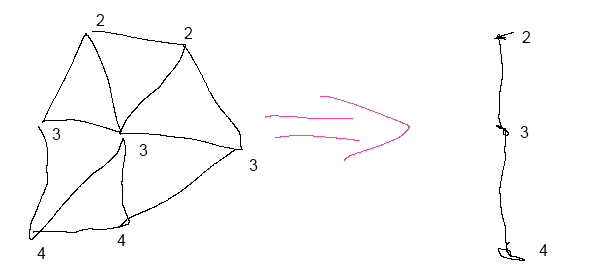
\includegraphics[width=0.88\textwidth]{collapse}
\caption{Collapsing cavity graph vertices.}
\label{fig:collapse}
\end{figure}

Finally, as the set of starting points we pick the vertices $v$ for which the condition $h(v) > h(u)$ holds for all neighbor vertices. Such vertices are illustrated in figure \ref{fig:start}.

\begin{figure}[h]
\centering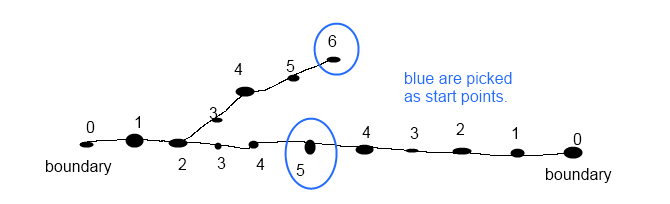
\includegraphics[width=0.88\textwidth]{start}
\caption{Starting points.}
\label{fig:start}
\end{figure}

\subsubsection{End Points}
Similar to the start points, end points are either user defined (by clicking on the boundary of the molecular surface) or calculated.

The calculation is very straighforward. For each cavity graph a subgraph $B$ is induced by the boundary vertices. All vertices that do no fit a probe with so called \textit{opening threshold} are removed. Then, strongly connected components of $B$ are computed. For each component, the vertex with the highest volume is picked as a tunnel end point.
\subsection{Tunnel Computation}

Now, having the start an end points, the tunnel calculation itself is very straightforward - Dijkstra's algorithm is used to compute the shortest paths between all pairs of start and end points. The function $w$ used for edge weights is the same as in the previous version:

\[
w(e)=\frac{l(e)}{d_c(e)^2+\epsilon},
\]

where $l(e)$ is the length of the edge, $d_c(e)$ is the distance to the closest van der Waals sphere, and $\epsilon$ is a small number to avoid division by zero.

\subsubsection{Representing the Tunnels}

The result of the Dijstra search is a set of tunnels each represented as a sequence of vertices. This is not a very desirable representation, therefore we fit a natural spline thru these points. Afterward, the spline is sampled and the several closest atoms, usually 10, are found for each point (actually, the closest point on the VDW sphere is found). These atoms are used to determine the radius of the tunnel at the given point and the list of surrounding residues. Information where the tunnel passes along the backbone is also provided. The sampling rate of the spline varies - it's 1.5 points per angstrom for visualization and 8 points per angstrom for tunnel profile (graph showing tunnel length and radius).

\subsection{Tunnel Comparison}

The tunnel comparison tool is used to mostly visually compare system of tunnel in different proteins. This works by letting the user select 3 residues which are used to align 2 or more proteins. After the proteins are aligned, a number representing the mutual distance of tunnels in the proteins is computed.

\subsubsection{Superimposing the Molecules}
The proteins are superimposed using 3 user selected residues. Centroids of these residues are used to align the molecules. To align 2 molecules, we use the quaternion based algorithm presented in \cite{something}. If multiple molecules are being compared, they are all superimposed to the first one.

\subsubsection{Tunnel distance}

DO THIS AS 2 POINT SET DISTANCE

Once the molecules are superimposed, we are ready to compare the tunnels. The comparison only takes into account the centerlines of the tunnels which is represented by a function $T:\rr \rightarrow \rr^3$ which maps the interval $<0, 1>$ onto points of the spline. We then define the so called \textit{directed tunnel distance} as
\[
\vec{d}(A, B) = \frac{\int_0^1\|A(t)-c_B(A(t)) \|^2\mathrm{d}t}{\|A\|},
\]
where $c_B(x)$ is the closest point on curve $B$ to the point $x$.

Because in general $\vec{d}(A, B)\not{=}\vec{d}(B, A)$ we define the \textit{tunnel distance} as
\[
d(A, B)=\frac{\vec{d}(A, B)+\vec{d}(B, A)}{2}
\]

To compute the function $d$ we approximate both curves using $N$ sample points (usually 4 points per angstrom) and the computation reduces to
\[
\vec{d}_N(A^N,B^N)=\frac{\sum_{i=1}^N \|A_i^N-c_B^N(A_i^N) \|^2}{\|A^N\|}
\]
and 
\[
d_N(A, B)=\frac{\vec{d}_N(A^N, B^N)+\vec{d_N}(B^N, A^N)}{2}
\]
respectively.

To compute the function $c^N_*$, $k$D-tree \cite{kdtree} of the curve is used.

If more than 2 molecules are compared, the average distance between all pairs is returned.

\bibliographystyle{amsalpha} % decsci, abbrvnat, ametsoc, amsalpha, unsrturl}
\bibliography{literature}


\end{document}
